\documentclass{scrartcl}
\usepackage{german}
\usepackage[utf8]{inputenc}
\usepackage[german]{babel}
\usepackage{amssymb}  % advanced mathematical symbold
\usepackage{graphicx} % using graphics
\usepackage{fancyhdr} % for the head of the page
\usepackage{lastpage} % makes page numbers work
\setlength{\parskip}{\medskipamount} % thats reasonable
\setlength{\parindent}{0pt}

% \usepackage{tikz}
% \usetikzlibrary{graphdrawing.layered}

%%%%%%%%%%%%%%%%%%%%%%%%
% Kopf- und Fusszeilen %
%%%%%%%%%%%%%%%%%%%%%%%%
\pagestyle{fancy}
\lhead{
    \begin{tabular}{ll}
        Felix Karg & 4342014\\
    \end{tabular}
}
\chead{Graphentheorie}
\rhead{
    \begin{tabular}{rr}
        \today{} \\
        Seite \thepage{} von \pageref{LastPage}
    \end{tabular}
}
\lfoot{}
\cfoot{}
\rfoot{}

%%%%%%%%%%%%%%%%%%%%%%%%
% Anfang des Dokuments %
%%%%%%%%%%%%%%%%%%%%%%%%
\begin{document}

\section*{Antworten zu Übungsblatt Nr. 2}

\section*{Aufgabe 1}
Frage: Welche der Folgenden Aussagen sind Äquivalent:
\begin{itemize}
    \item $G$ enthält einen einfachen Kreis
    \item $G$ enthält einen elementaren Kreis
    \item $G$ enthält einen Kreis
\end{itemize}

Kreis: \\
Pfad, mit gleichem Start und Endpunkt \\

einfacher Kreis: \\
Kreis, in dem Kanten nicht mehrfach begangen werden \\

elementarer Kreis: \\
Kreis, in dem weder Kanten noch Knoten mehrfach begangen werden \\

Dementsprechend enthält jeder Graph Kreise. Äquivalent sind die Aussagen nun
nur für gerichtete Graphen, da sonst o-o ein Kreis, aber weder einfach noch
elementar wäre. \\
Äquivalent sind sie mit Folgender Begründung: solange G gerichtet ist und einen
Kreis enthält kann man ihn zu einem elementaren 'kürzen' (falls notwendig),
wodurch er auch einfach ist, dementsprechend 'enthält' G, sobald er mindestens
einen Kreis enthält, auch einfache und elementare.


\section*{Aufgabe 2}

Frage: \\
Betrachten Sie einfache ungerichtete Graphen:
\begin{itemize}
    \item[1] Gibt es einen 3-regulären Graphen mit $n = 7$ Ecken?
    \item[2] Sind alle 3-regulären Graphen mit $n = 4$ Ecken
        jeweils Isomorph zueinander? Wie sieht es bei $n = 6$
        aus?
\end{itemize}

n-regulär heißt, dass an jedem Knoten genau n ausgehende verbindungen sind.

\begin{itemize}
    \item[1] Nein, es müsste insgesamt $(3 * 7 = ) 21$ Aus- bzw. Eingänge
        geben, da dies aber eine ungerade Zahl und daher nicht möglich ist ist
        ein solcher Graph nicht möglich.
    \item[2] Ja, da es keine Schlingen (einfach, ungerichtet) gibt für $n = 4$,
        also jeweils drei ausgehende auf die anderen Knoten abgebildet werden
        müssen. Bei $n = 6$ sieht es anders aus, da hier durchaus mehr
        möglichkeiten bestehen die nicht nur Permutationen sind, sondern sich
        wirklich nicht ineineander überführen lassen, also nicht isomorph sind.
\end{itemize}

\section*{Aufgabe 3}

Betrachten sie Folgende Graphen, Zeichnen sie die Line-Graphen
dafür. Gibt es für i = 1, 2, 3 einen Graphen $H_i$ mit $L(H_i) =
G_i$? Begründen Sie jeweils ihre Antwort. \\ \\

% \tikz [layered layout] {
%     a -- b -- c -- a
% }

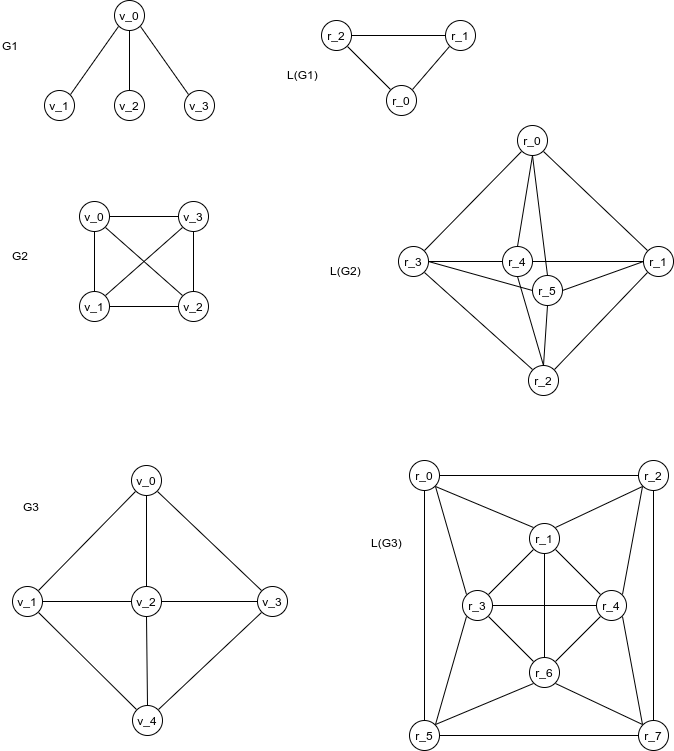
\includegraphics[width=14cm]{Graphs.png}

$H_1$: kann es nicht geben, da man hier drei Kanten bräuchte, die alle über
eine Kante verbunden sind, aber nicht untereinander, was für zwei noch
Funktioniert aber nicht für mehr, wenn die Kante nur mit zwei Knoten verbunden
sein darf. \\
$H_2$: Es gibt mindestens eine Möglichkeit mit schleifen, und zwar in dem ein
Knoten, $v_0$, Vier davon hat (oder ähnlich). Andernfalls wird es schwierig,
die jeweils Diagonalen zu verbinden. \\
$H_3$: Existiert, ist fast $G_2$, bis auf eine der beiden Diagonalen.


\end{document}


Beispiel für Text, der aus einem Terminal kopiert wurde:

\begin{verbatim}
osswald@tfpool17 / $ df -h
Filesystem                           Size  Used Avail Use% Mounted on
/dev/sda4                            375G   41G  316G  12% /
dev                                  3.9G     0  3.9G   0% /dev
run                                  3.9G  480K  3.9G   1% /run
tmpfs                                3.9G     0  3.9G   0% /dev/shm
\end{verbatim}

Aufzählungen sind mit \verb_enumerate_ möglich:
\begin{enumerate}
\item Erster Punkt
\item Zweiter Punkt
\item Dritter Punkt
\end{enumerate}

\subsection*{Aufgabe 2}

Mathematische Formeln:
\begin{equation}\label{gauss}
    \sum_{i=1}^{n} i = \frac{n(n+1)}{2}
\end{equation}


Formel \ref{gauss} wird auch \emph{Gaußsche Summenformel} genannt.

Formeln können auch im Text eingebunden werden, z.B. $E = mc^{2}$.

\subsection*{Aufgabe 3}

Tabellen können mit \verb_tabular_-Umgebungen eingegeben werden:

\begin{center}
\begin{tabular}{l|l|l}
Datei             & Dateirechte        & Größe   \\
\hline
dokument.txt      & \verb_-rw-r--r--_  & 300 KB  \\
programm.exe      & \verb_-rwxr-x---_  & 450 KB  \\
mein\_verzeichnis & \verb_drwxr-xr-x_  & ---     \\
\end{tabular}
\end{center}

\end{document}


